\newcommand{\AppendixSetup}{%
  \appendix
  \renewcommand{\thesection}{\Alph{section}} % A/B/C...
  \setcounter{tocdepth}{2}\setcounter{secnumdepth}{2}

  % 章节标题样式
  \titleformat{\section}{\large\bfseries\color{red}}{\thesection}{1em}{}
  \titleformat{\subsection}{\normalsize\bfseries}{\thesubsection}{0.8em}{}

  % 附录目录条目样式(点线 + 右对齐页码)
  \titlecontents{section}
    [0em]{\bfseries\color{red}}{\contentslabel{1.2em}}{}{\titlerule*[.5pc]{.}\contentspage}[\vspace{0.2em}]
  \titlecontents{subsection}
    [1.8em]{}{\contentslabel{1.6em}}{}{\titlerule*[.5pc]{.}\contentspage}[\vspace{0.1em}]
}

\newcommand{\AppendixTitlePage}{%
  \begin{center}
    \LARGE\bfseries Appendix\par
  \end{center}
  \vspace{0.75em}
  \noindent\textbf{Contents}\par
  \vspace{0.5em}
}

% ===== 第一页只放目录 =====
\clearpage
\AppendixSetup
\startcontents[app]          % 开始捕获“附录目录”
\AppendixTitlePage
\printcontents[app]{l}{1}{}  % 打印仅附录目录(section+subsection)
\clearpage                   % ← 目录页结束;正文从新页开始

% ====== 你的附录正文 ======
\section{Checklist}
\subsection{The Use of Large Language Models}
In our work, LLMs are used for following aspects:
\begin{itemize}
    \item Using an LLM to help with paper writing. We use GPT5 to help optimize language, correct grammar and write {\LaTeX} table code.
    \item Using an LLM as a research assistant. We use GPT5 to help search related works.
    \item Using an LLM in our methods and experiment. This is described in the paper.
\end{itemize}
\subsection{Ethics Statement}
We confirm that our study did not use any sensitive data where all data are public available. We have conducted this research and reported our findings responsibly. All results are presented transparently, including both performance gains and any observed limitations. We have diligently cited all relevant prior work and data sources to give proper credit and context. By following best practices in documentation and research integrity, we aim to contribute positively to the scientific community while upholding the highest ethical standards.
\subsection{Reproducibility statement}
We are committed to ensuring the reproducibility of our results. All code and data needed to reproduce the experiments will be made publicly available. We will release this repository openly with an appropriate open-source license upon publication. The datasets used in our experiments are standard public benchmarks for language modeling and understanding (e.g., widely-used corpora and evaluation sets). These resources are readily accessible to other researchers.
% \section{PaperTalker}
% The details of repair and visual-selective MCTS layout refinement are shown in Algorithm~\ref{alg:compile-repair} and Algorithm~\ref{alg:visual-selective} respectively.
% \begin{algorithm}
% \small
% \caption{Slide Generation via Compile--Repair}
% \label{alg:compile-repair}
% \begin{algorithmic}[1]
% \Require Text source $t$; figure set $\mathcal{F}=\{f_i\}_{i=1}^{n}$; max iterations $K$
% \Ensure Compilable slide code $c^{*}$
% \State $c \gets \operatorname{LLM}(t, \mathcal{F})$ \Comment{initial draft $c^{(0)}$}
% \For{$k = 1$ \textbf{to} $K$}
%     \State $(e, w) \gets \operatorname{Compile}(c)$
%     \If{$e = \varnothing$}
%         \State $c^{*} \gets c$; \Return $c^{*}$ \Comment{no errors; stop}
%     \EndIf
%     \State $c \gets \operatorname{LLM}(c, e)$ \Comment{repair using compiler errors only}
% \EndFor
% \State $c^{*} \gets c$; \Return $c^{*}$ \Comment{best-effort if max iterations reached}
% \end{algorithmic}
% \end{algorithm}

% \begin{algorithm}
% \footnotesize
% \caption{Visual-Selective Layout Refinement}
% \label{alg:visual-selective}
% \begin{algorithmic}[1]
% \Require Compilable slide code $c^*$; text font scales $\mathcal{A}_{\text{text}}$; figure font scale $\alpha_{\text{fig}}$; figure scales $\mathcal{B}$
% \Ensure Refined slide code $c^{\dagger}$ and slides $s$
% \State $(\_, w)\gets\operatorname{Compile}(c^*)$;\ \ $\mathcal{I}\gets\operatorname{OverfullFrames}(w)$
% \If{$\mathcal{I}=\varnothing$} \State \Return $c^{\dagger}\gets c^*$ \EndIf
% \For{\textbf{each } $i\in\mathcal{I}$}
%   \State $s\gets\operatorname{ExtractFrame}(c^*,i)$;\ \ $\mathcal{C}\gets\varnothing$
%   \If{$\operatorname{IsTextOnly}(s)$}
%     \State $\mathcal{C}\gets\{\operatorname{ApplyFontScale}(s,\alpha):\alpha\in\mathcal{A}_{\text{text}}\}$
%   \Else
%     \State $s_{\text{font}}\gets\operatorname{ApplyFontScale}(s,\alpha_{\text{fig}})$
%     \State $\mathcal{C}\gets\{s_{\text{font}}\}\ \cup\ \{\operatorname{ApplyFigureScale}(s_{\text{font}},\beta):\beta\in\mathcal{B}\}$
%   \EndIf
%   \State $\text{img}\gets\{\operatorname{RenderAsImage}(c \text{ with } s' \text{ at } i): s'\in\mathcal{C}\}$
%   \State $s^{\star}\gets\arg\max_{s'\in\mathcal{C}}\ \operatorname{VLM\_Judge}(\text{img}[s'],\text{prompt}_{\text{layout}})$
%   \State $c\gets\operatorname{ReplaceFrame}(c,i,s^{\star})$
% \EndFor
% \State $c^{\dagger}\gets c$
% \State \Return $s\gets\operatorname{CompilePDF}(c^{\dagger})$
% \end{algorithmic}
% \end{algorithm}

\section{Evaluation Metrics}
\subsection{IP Memory}
\label{sec:ip}
We propose a novel metric to evaluate how well an audience retains a work after watching its presentation video. Motivated by \textbf{real-world conference interactions}, this metric assesses whether an audience member, after viewing several presentation videos, can recall the work and pose a relevant question when meeting the author.

To operationalize this, we construct video–question pairs by sampling a five-second clip from each presentation video and selecting a corresponding understanding-level question from PresentQuiz. A VideoLLM serves as the audience proxy: it is presented with four randomly sampled video–question pairs, where the videos and questions are shuffled, together with an image of one speaker as the query. The model is then asked to identify the relevant question to pose, and the accuracy quantifies the IP Memory score. Higher recall accuracy indicates that the generated results are more impressive and hold greater potential for lasting impact.



\section{Experiment}
\subsection{Video Results}
Video results please refer to the supplementary materials.

\subsection{Results of Tree Search Visual Choice}
Figure~\ref{fig:tree_vis} illustrates the slides before and after applying tree search visual choice refinement. The refinement \textbf{resolves the overfull issues} and substantially improves slide quality, indicating that this module \textbf{plays a crucial role in layout adjustment}.
\begin{figure}[t]
    \centering
    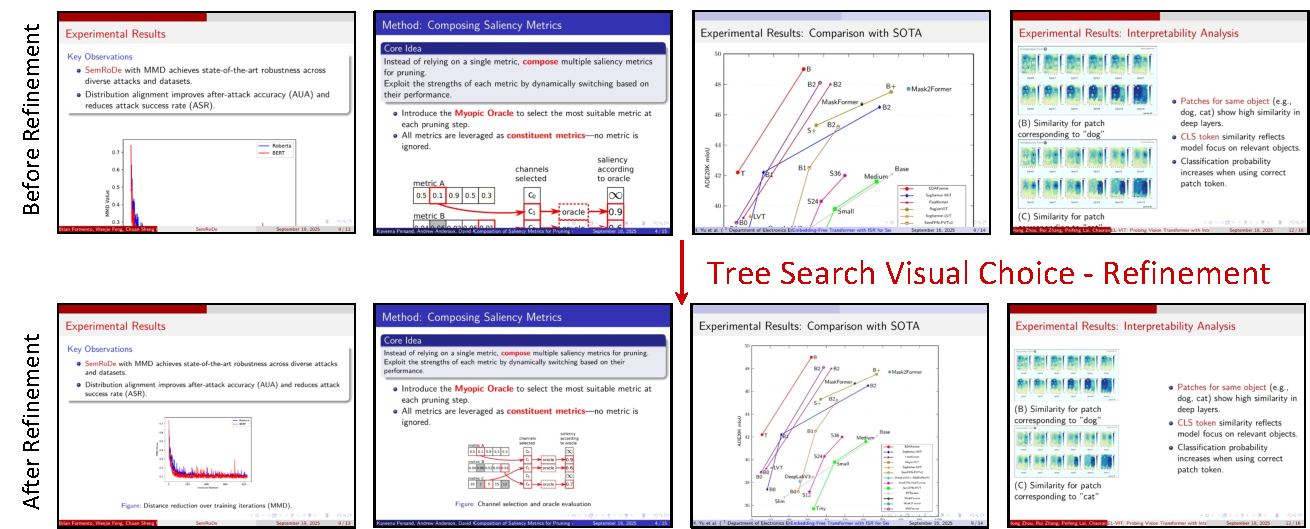
\includegraphics[width=\linewidth]{figure/tree_search_vis.pdf}
    \caption{\textbf{Slide Visualization of Tree Search Visual Choice.} The first row shows slide results before layout refinement, while the second row shows their corresponding slides after refinement.}
    \label{fig:tree_vis}
\end{figure}

\section{Prompts}
% 颜色(可按需调整)
\definecolor{CardHeader}{RGB}{124,146,84}  % 橄榄绿标题栏
\definecolor{CardHeaderDark}{RGB}{100,120,65}
\definecolor{CardFrame}{RGB}{205,210,190}  % 浅绿边框

% 小圆点
\newcommand{\headerdot}{\tikz[baseline=-0.6ex]\node[circle,fill=CardHeaderDark,inner sep=1.5pt]{};}

% 卡片环境
\newtcolorbox{promptbox}[1]{%
  enhanced, breakable,
  colback=white, colframe=CardFrame,
  boxrule=0.5pt, arc=2mm,
  left=10pt,right=10pt,top=8pt,bottom=10pt,
  before skip=8pt, after skip=10pt,
  drop shadow=black!15,
  attach boxed title to top left={xshift=1mm,yshift*=-2mm},
  boxed title style={
    colback=CardHeader, colframe=CardHeader, coltext=white,
    boxrule=0pt, left=8pt,right=8pt,top=3pt,bottom=3pt, arc=2mm
  },
  title={\headerdot\ \textbf{Prompt:}~#1},
}

\begin{promptbox}{Slide Generation}
\textbf{System Prompt:} Please generate a complete English PPT introduction based on the following TeX source text content, using LaTeX Beamer. The specific requirements are as follows.

\medskip
\textbf{Content structure:}
\begin{itemize}[leftmargin=1.2em,itemsep=2pt,topsep=2pt]
  \item The PPT should contain the following chapters (arranged in order), and each chapter must have a clear title and content:
  \item Motivation (research background and problem statement)
  \item Related work (current status and challenges in the field)
  \item Method (core technical framework) [The content of the method needs to be introduced in detail, and each part of the method should be introduced on a separate page]
  \item Innovation (differentiation from existing work)
  \item Experimental method (experimental design and process)
  \item Experimental setting (dataset, parameters, environment, etc.)
  \item Experimental results (main experimental results and comparative analysis)
  \item Ablation experiment (validation of the role of key modules)
  \item Deficiencies (limitations of current methods)
  \item Future research (improvement direction or potential application)
  \item End slide (Thank you)
\end{itemize}

\textbf{Format requirements:}
\begin{itemize}[leftmargin=1.2em,itemsep=2pt,topsep=2pt]
\item Use Beamer's theme suitable for academic presentations, with simple color matching.
\item The content of each page should be concise, avoid long paragraphs, and use itemize or block environment to present points.
The title page contains the paper title, author, institution, and date.
\item Key terms or mathematical symbols are highlighted with \text{\\alert\{\}}.
\end{itemize}

\textbf{Image and table processing:}
\begin{itemize}[leftmargin=1.2em,itemsep=2pt,topsep=2pt]
\item All image paths are given, and relative paths are used when citing, the picture names must "be consistent with the name in tex file".
\item Images should automatically adapt to width, and add titles and labels
\item Experimental result tables should be extracted from the source text, formatted using tabular or booktabs environments, and marked with reference sources ( "as shown in table").
\end{itemize}

\textbf{Code generation requirements:}
\begin{itemize}[leftmargin=1.2em,itemsep=2pt,topsep=2pt]
\item The generated LaTeX code must be complete and can be compiled directly (including necessary structures).
\item Mark the source text location corresponding to each section in the code comments (for example, % corresponds to the source text Section 3.2).
\item If there are mathematical formulas in the source text, they must be retained and correctly converted to LaTeX syntax (such as $y=f(x)$).
\end{itemize}

\textbf{Other instructions:}
\begin{itemize}[leftmargin=1.2em,itemsep=2pt,topsep=2pt]

\item Image content should be read from the tex file, and the source name should be used directly without arbitrary modification. Image references should use real image names and should not be forged;
\item Table content should first extract real data from the source document.
\item All content should be in English.
\item If the source text is long, it is allowed to summarize the content, but the core methods, experimental data and conclusions must be retained.
\item To enhance readability, a transition page can be added (for example, "This section will introduce the experimental part").
\item Perfer more images than heavy text. **The number of slides should be around 10.** 
\item **\& in title is not allowed which will cause error "Misplaced alignment tab character \&\"**
**Pay attention to this "error: !File ended while scanning use of \text{\\frame}\"**
\item Only output latex code which should be ready to compile using tectonic(simple verson of TeX Live). Before output check if the code is grammatically correct.
\end{itemize}
\end{promptbox}

\begin{promptbox}{Error Correction}
\textbf{System Prompt:} You are given a LaTeX Beamer code for the slides of a research paper and its error information. Correct these errors \emph{without changing} the slide content (text, figures, layout).

\medskip
\textbf{Instructions:}
\begin{itemize}
  \item Apply the minimal edits required to make the file compile: add missing packages, close/open environments, balance braces, escape special characters, fix math delimiters, resolve duplicate labels, and correct obvious path or option typos.
  \item Do \emph{not} paraphrase or delete text; do \emph{not} change figure/table content, captions, labels, or layout semantics.
  \item Keep all image/table file names and relative paths as given; do not invent or rename assets.
  \item Preserve the original Beamer theme, colors, and structure.
  \item Ensure the final output compiles with \textbf{Tectonic}; close all environments and avoid undefined commands.
\end{itemize}

\medskip
\textbf{Output (strict):} Output \emph{only} the corrected LaTeX source, beginning with \texttt{beamer} and ending with \texttt{document}; no extra commentary.
\end{promptbox}

% 上面一行的说明文字(如截图左上角的粗体句子)
\begin{promptbox}{MSTS Judge}
\textbf{System Prompt:} You are a slide layout judge. You see four slides A–D in a 2×2 grid:
A (top-left), B (top-right), C (bottom-left), D (bottom-right).

\medskip
\textbf{Definitions}
\begin{itemize}[leftmargin=1.2em,itemsep=2pt,topsep=2pt]
  \item \textbf{Overfull:} any part of the figure or its caption is clipped, outside the frame, or overlapped/hidden.
  \item \textbf{Coverage:} among non-overfull options, larger visible content with less empty background is better.
  \item \textbf{Risk:} risk of overfull decreases from A → D (A largest, D smallest).
  \item \textbf{Coverage trend:} coverage decreases from A → D.
\end{itemize}

\textbf{Rules (judge only the given images)}
\begin{enumerate}[leftmargin=1.2em,itemsep=2pt,topsep=2pt]
  \item Disqualify any option with overfull (caption must be fully visible).
  \item From the remaining, pick the one with the greatest coverage.
  \item Practical method: scan \textbf{A → B → C → D}; choose the \emph{first} slide in that order that is not overfull.
\end{enumerate}

\medskip
\textbf{Output only (strict; do \emph{not} output \texttt{```json}):}
\begin{verbatim}
{
"reason": "concise comparison",
"choice": "A" | "B" | "C" | "D"
}
\end{verbatim}
\end{promptbox}


\begin{promptbox}{Slide Script with Cursor Positions}
\textbf{System Prompt:} You are an academic researcher presenting your own work at a research conference. You are provided with a sequence of adjacent slides.

\medskip
\textbf{Instructions:}
\begin{itemize}[leftmargin=1.2em,itemsep=2pt,topsep=2pt]
  \item For each slide, write a smooth, engaging, and coherent first-person presentation script.
  \item Clearly explain the \emph{current} slide with academic clarity, brevity, and completeness; use a professional, formal tone and avoid content unrelated to the paper.
  \item Each sentence must include \emph{exactly one} cursor position description drawn from the \emph{current slide} and listed in order, using the format \texttt{script\;|\;cursor description}. If no cursor is needed for a sentence, write \texttt{no}.
  \item Limit the total script for each slide to \textbf{50 words} or fewer.
  \item Separate slides using the delimiter \texttt{\#\#\#}.
\end{itemize}

\medskip
\textbf{Output Format (strict):}
\begin{verbatim}
sentence 1 | cursor description
sentence 2 | cursor description
...
###
sentence 1 | cursor description
...
\end{verbatim}
\end{promptbox}


\begin{promptbox}{Meta Similarity}
\textbf{System Prompt:} You are an evaluator. You will be given two presentation videos of the same talk: (1) a human-presented version and (2) an AI-generated version. Evaluate \emph{only} the slides and subtitles; ignore the presenter’s face, voice quality, background music, camera motion, and any non-slide visuals.

\medskip
\textbf{Inputs You May Receive}
\begin{itemize}[leftmargin=1.2em,itemsep=2pt,topsep=2pt]
  \item Human video (and optionally its slide images and subtitles/transcript)
  \item AI video (and optionally its slide images and subtitles/transcript)
\end{itemize}

\textbf{Evaluation Scope (focus strictly on slides + subtitles)}
\begin{enumerate}[leftmargin=1.2em,itemsep=2pt,topsep=2pt]
  \item \textbf{Slide Content Matching:} Do AI slides convey the same key points and comparable layout/visual elements (titles, bullets, diagrams, tables, axes annotations) as the human version?
  \item \textbf{Slide Sequence Alignment:} Is slide order consistent? Any sections missing, added, or rearranged?
  \item \textbf{Subtitle Wording Similarity:} Do AI subtitles reflect similar phrasing/terminology and information as the human speech/subtitles? Focus on semantic equivalence; minor style/spelling differences do not matter.
  \item \textbf{Slide–Subtitle Synchronization:} Within the AI video, does narration/subtitle content match the on-screen slide at the same time? Does this broadly align with the human presenter’s per-slide content?
\end{enumerate}

\textbf{Evidence-Only Rules}
\begin{itemize}[leftmargin=1.2em,itemsep=2pt,topsep=2pt]
  \item Base the judgment solely on the provided materials (videos, slides, subtitles). Do \emph{not} use outside knowledge.
  \item If some inputs are missing (\textit{e.g.}, no subtitles), judge from what is available and briefly note the missing piece in the Reasons.
\end{itemize}

\textbf{Relaxed Scoring Rubric (0–5)}
\begin{itemize}[leftmargin=1.2em,itemsep=2pt,topsep=2pt]
  \item \textbf{5} — Nearly identical: slides and subtitles closely match the human version in content, layout, sequence, and timing; wording is near-paraphrase.
  \item \textbf{4} — Highly similar: only minor layout/phrasing differences; content, order, and alignment clearly match.
  \item \textbf{3} — Moderate differences yet same core content: several layout/wording/sequence deviations but main sections and key points are preserved. (Leniency: borderline cases between 2 and 3 \emph{round up} to 3.)
  \item \textbf{2} — Partial overlap: substantial omissions/rearrangements or subtitle drift; multiple slide mismatches or sync issues.
  \item \textbf{1} — Minimal overlap: only a few matching fragments; most slides/subtitles diverge.
  \item \textbf{0} — No meaningful match: AI slides/subtitles do not correspond to the human version.
\end{itemize}
\noindent\emph{Lenient mapping: if borderline between adjacent levels, choose the higher score. If computing subscores, average and \textbf{round up} to the nearest integer in [0,5].}

\medskip
\textbf{Output Format (STRICT; exactly one line)}
\begin{verbatim}
Content Similarity: X/5; Reasons
\end{verbatim}
Where \texttt{X} is an integer 0–5 from the rubric, and \texttt{Reasons} is 1–3 short sentences referencing content, sequence, wording, and synchronization as relevant.
\end{promptbox}


\begin{promptbox}{PresentArena}
\textbf{System Prompt:} You are an expert in evaluating academic presentation videos. You are given two videos (Video A and Video B) on the same research topic. Evaluate each video independently and then decide which is better, or if they are basically the same (preferred when not confident).

\medskip
\textbf{Evaluation Criteria}
\begin{itemize}[leftmargin=1.2em,itemsep=2pt,topsep=2pt]
  \item \textbf{Content Clarity}: Are key ideas and findings clearly explained?
  \item \textbf{Speaker Delivery}: Is the speaker confident, fluent, and engaging?
  \item \textbf{Visual Aids}: Are slides/visuals clear, helpful, and well-integrated?
  \item \textbf{Structure \& Pacing}: Is the talk logically organized and appropriately paced?
  \item \textbf{Audience Engagement}: Does the speaker maintain interest and attention?
\end{itemize}

\textbf{Steps}
\begin{enumerate}[leftmargin=1.2em,itemsep=2pt,topsep=2pt]
  \item \textbf{Step 1:} Write a short (1–2 sentence) evaluation of \textbf{Video A} based on the criteria.
  \item \textbf{Step 2:} Write a short (1–2 sentence) evaluation of \textbf{Video B} based on the criteria.
  \item \textbf{Step 3:} Decide which video is better, or if they are basically the same (prefer ``Same'' if not confident).
\end{enumerate}

\medskip
\textbf{Output Format (Strict; only these three blocks):}
\begin{verbatim}
Step 1:
[1–2 sentences evaluating Video A]

Step 2:
[1–2 sentences evaluating Video B]

Step 3:
Final Judgment:
[A] | [B] | [Same]

Reason: [One concise sentence justifying the judgment based on Steps1-2.]
\end{verbatim}
\end{promptbox}


\begin{promptbox}{PresentationQuiz}
\textbf{System Prompt:} You are an answering agent. You will be provided with:
1) a presentation video of a paper, and 2) a JSON object called \texttt{"questions"} containing multiple questions, each with four options (A–D).
Analyze the video thoroughly and answer each question \emph{solely} based on the video content (no external knowledge). Do not reference timesteps that exceed the video length.

\medskip
\textbf{Instructions:}
\begin{itemize}
  \item For each question, if the video provides sufficient evidence for a specific option (A, B, C, or D), choose that option.
  \item Include a brief reference to where in the video the evidence appears (\textit{e.g.}, ``Top-left text'', ``Event date section'').
  \item Rely only on the video; do not use outside context.
  \item Provide an answer entry for \emph{all} questions present in \texttt{"questions"}.
\end{itemize}

\medskip
\textbf{Template (steps to follow):}
\begin{enumerate}
  \item Study the presentation video together with \texttt{"questions"}.
  \item For each question, determine whether the video clearly supports one of the four options; if so, pick that answer.
  \item Provide a brief reference indicating where in the video you found the evidence.
  \item Format the final output strictly as a JSON object with the following pattern (and no extra keys or explanations).
\end{enumerate}

\textbf{Output Format (strict):}
\begin{verbatim}
{
  "Question 1": { "answer": "X", "reference": "some reference" },
  "Question 2": { "answer": "X", "reference": "some reference" },
  ...
}
\end{verbatim}

\textbf{questions payload:}
\begin{verbatim}
{{questions}}
\end{verbatim}
\end{promptbox}

